\documentclass[journal]{IEEEtran}
\ifCLASSINFOpdf \else \fi
\usepackage{graphicx}
% *** MATH PACKAGES ***
\usepackage[cmex10]{amsmath}
\usepackage{amssymb}
% *** Algorithm PACKAGES ***
\usepackage{algorithmic}
% *** ALIGNMENT PACKAGES ***
\usepackage{array}
% *** SUBFIGURE PACKAGES ***
\ifCLASSOPTIONcompsoc
 \usepackage[caption=false,font=normalsize,labelfont=sf,textfont=sf]{subfig}
\else
 \usepackage[caption=false,font=footnotesize]{subfig}
\fi
% *** PDF, URL AND HYPERLINK PACKAGES ***
\usepackage{url}
%
% correct bad hyphenation here
\hyphenation{caratteris-tiche dispo-sitivi}
\usepackage[noadjust]{cite}

\begin{document}

\title{Assorbimento di una MQW in Ge/SiGe con barriere 
ad alto contenuto di Ge}

\author{Onofrio Davide Caputo, Elsaid Meaj, Adriano Notarangelo
    \\ Università degli Studi di Milano Bicocca}

\maketitle

% As a general rule, do not put math, special symbols or s
% in the abstract or keywords.
\begin{abstract}
L’obiettivo del paper è quello di studiare le proprietà ottiche mediante esperimenti di assorbimento di dispositivi costituiti da una successione di pozzi quantici (Multiple Quantum Wells) con buche in Germanio e barriere in lega Silicio/Germanio ad alto contenuto di Germanio, compensate in strain.
Le caratteristiche degli spettri evidenziano un ottimo comportamento del Germanio come assorbitore nella regione spettrale dell'IR. Tali proprietà forniscono la possibilità di utilizzare dispositivi di questo tipo nella costruzione di modulatori ottici.

\end{abstract}

% \begin{IEEEkeywords}
% IEEEtran, journal, \LaTeX, paper, template.
% \end{IEEEkeywords}

\IEEEpeerreviewmaketitle

\section{Introduzione}

È possibile realizzare un dispositivo costituito da una successione di pozzi quantici 
(Multiple Quantum Wells) utilizzando etero-giunzioni nelle quali vanno ad interfacciarsi due diversi semiconduttori in maniera alternata.
Per avere una struttura che possieda buone proprietà ottiche in assorbimento (alto coefficiente di assorbimento) e in emissione è necessario che l'allineamento di banda nelle etero-giunzioni sia di tipo I, infatti ciò garantisce che elettroni e lacune siano intrappolati nello stesso strato, favorendo le transizioni radiative. Inoltre si predilige l'utilizzo di semiconduttori a gap diretto (o con proprietà simili ad essi) per costruire i pozzi quantici, in modo da massimizzare la probabilità delle transizioni elettroniche radiative interbanda nella regione spettrale dell'IR.


\section{Costruzione e caratteristiche della MQW}

Nel caso in analisi si considera una struttura in cui i pozzi quantici sono costruiti in Germanio, il quale cresce sotto strain compressivo, mentre le barriere sono costruite in lega tra Silicio e Germanio, che cresce sotto strain tensile.

Poiché si vuole avere compatibilità di tale dispositivo con tutti quelli utilizzati in microelettronica, si costruisce la successione di pozzi quantici a partire da un substrato di Silicio, largamente utilizzato nella suddetta industria.
Il Silicio non può essere direttamente impiegato all'interno della MQW per realizzare i pozzi quantici, in quanto sottili strati di tale materiale risultano essere praticamente trasparenti nella regione spettrale dell'IR, come conseguenza delle caratteristiche della sua struttura a bande.
Infatti il Silicio è un semiconduttore a gap indiretto, quindi le transizioni elettroniche radiative tra il massimo della banda di valenza e il minimo della banda di conduzione sono statisticamente poco probabili poiché richiedono un'interazione in cui sono coinvolti tre corpi (elettrone, fotone e fonone), rendendo il coefficiente di assorbimento del Silicio nella regione spettrale dell'IR molto basso (l'energy gap diretto del Silicio è pari a 3.5 eV, quindi nell'IR non sono possibili transizioni dirette).

La scelta del semiconduttore con il quale costruire i pozzi quantici del dispositivo ricade quindi sul Germanio, che possiede la stessa struttura reticolare del Silicio (diamante) e proprietà ottiche notevolmente migliori nella regione IR. Ciò è determinato dal fatto che, nonostante il Germanio sia un semiconduttore a gap indiretto (per cui il minimo assoluto della banda di conduzione si osserva in posizione L), esso presenta un minimo relativo della banda di conduzione in posizione $\Gamma$, che differisce solamente di circa $0.14$ eV dal minimo assoluto ($E_L$ = 0.661 eV, $E_\Gamma$ = 0.80 eV) a temperatura ambiente (T = 300 K). Ciò porta il Germanio ad avere caratteristiche simili ad un semiconduttore a gap diretto, garantendo buone propietà ottiche in assorbimento nella regione spettrale di interesse.

\begin{figure}[h!]
    \centering
    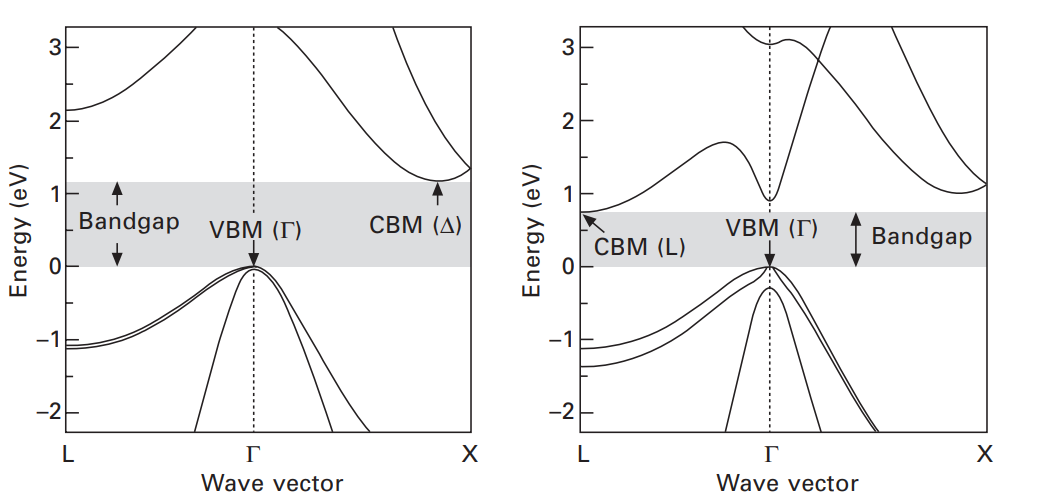
\includegraphics[width=\linewidth]{Images/Si&Ge_BandStructure.png}
    \caption{Struttura a bande del Silicio (sinistra) e del Germanio (destra).}
    \label{fig:my_label}
\end{figure}

Nonostante cristalli di Silicio e Germanio possiedano una struttura reticolare di tipo diamante, essi differiscono nel passo reticolare: esso nel Silicio è di 5.43 $\AA$ mentre nel Germanio è di 5.66 $\AA$. A causa di tale mismatch reticolare, nel momento in cui si deposita uno strato di Germanio su un substrato di Silicio, benché il primo si adatti inizialmente al passo reticolare del secondo crescendo sotto strain compressivo, una volta depositati quattro monolayers atomici, il Germanio tende a ritornare al suo passo reticolare naturale, a causa della notevole forza elastica, nucleando un'alta concentrazione di difetti di dislocazione ($\sim$ $10^8$ cm$^{-2}$) dannosi per il funzionamento del dispositivo.

Come conseguenza di ciò si ricorre all'utilizzo della tecnica dei substrati virtuali (VS) per poter adattare gradualmente il passo reticolare del Silicio a quello del Germanio, riducendo significativamente la concentrazione di difetti nel cristallo. Tale tecnica prevede, nel caso di interesse, la deposizione, a partire dal substrato di Silicio puro, di una lega tra Silicio e Germanio, in cui la concentrazione molare di Germanio aumenta linearmente con lo spessore dello strato depositato fino ad arrivare ad un valore finale in cui la lega presenta un alto contenuto di Germanio. In questo modo, depositando lo strato di Germanio puro a partire dal terminale del VS, il mismatch reticolare è notevolmente ridotto e si possono costruire strati di Germanio molto più spessi, i quali crescono sotto strain compressivo, adattandosi al passo reticolare del VS. Nella MQW gli strati di Germanio puro costituiscono i pozzi quantici, mentre le barriere vengono realizzate in lega Silicio/Germanio con un'alta concentrazione di Germanio. Tale concentrazione nelle barriere deve risultare minore rispetto a quella del terminale del VS, in modo che esse crescano sotto strain tensile. Calibrando opportunamente gli spessori dei pozzi e delle barriere si può ottenere una compensazione in strain che permette, idealmente, di costruire una successione infinita di pozzi e barriere in maniera alternata, ottenendo così una MQW in cui si mantiene bassa la concentrazione di difetti reticolari.

I campioni in analisi sono il 7909-3 e 7909-8 bilucidi, costituiti da una successione di 200 QW, in cui i pozzi sono in Ge puro, le barriere sono in lega Si/Ge con una concentrazione molare di Ge pari a 0.87 e la concentrazione molare di Ge al terminale del VS è pari a 0.89. La larghezza dei pozzi e delle barriere è nell'ordine della decina di nm.

I campioni sono stati realizzati utilizzando la tecnica di deposizione e crescita epitassiale Low-Energy Plasma-Enhanced Chemical Vapor Deposition (LEPECVD), la quale permette di ottenere un deposito, a partire da un precursore molecolare introdotto in forma gassosa, sulla superficie di un substrato solido introdotto nella camera del reattore in condizioni di UHV.
La tecnica LEPECVD permette di ottenere alti tassi di deposizione. I campioni in analisi sono stati cresciuti con un tasso di deposizione di 4-6 nm/s.


\section{Apparato Sperimentale}

Le misure di assorbimento ottico dei campioni in questione sono state portate a termine a temperatura ambiente nel laboratorio (300 K) mediante l'utilizzo di uno spettrometro a trasformata di Fourier Jasco FT/IR-800 equipaggiato con un rivelatore in InGaAs.

Nel sistema è presente una sorgente ad ampio spettro (lampada), che emette radiazione elettromagnetica, la quale viene collimata mediante un primo specchio per poi essere separata da un beam splitter (BS) in due fasci diretti su due diversi specchi, uno fisso e uno mobile, che riflettono indietro la luce generando una differenza di cammino ottico tra i due fasci, introducendo fenomeni di interferenza. Il fascio emergente dall'interferometro viene collimato da successivi specchi e fatto incidere sul campione. La radiazione emergente dal campione viene raccolta dal rilevatore. Durante un singolo scan lo specchio mobile si muove avanti e indietro rispetto al BS. In base alla differenza di cammino ottico dei due fasci, si ha interferenza costruttiva o distruttiva per le diverse componenti spettrali della radiazione. Si ottiene un interferogramma (intensità in funzione della differenza di cammino ottico) comprensivo di tutte le componenti spettrali della radiazione rivelata dal detector, che viene convertito, mediante la trasformata di Fourier, in un segnale in frequenza.
Nel set-up è presente anche una sorgente laser a He-Ne(caratterizzato da una lunghezza d'onda pari a $\lambda = 632.8 nm$) utilizzato per tarare l'interferometro di modo che gli spostamenti effettuati sullo specchio mobile siano misurabili mediante le figure di diffrazione generate dalla sorgente laser ed osservate da un fotodiodo presente nell'apparato stesso.

\begin{figure}[h!]
    \centering
    \includegraphics[width=\linewidth]{Images/FTIR_SpectrometerScheme.png}
    \caption{Schema dello spettrometro Jasco FT/IR-800.}
    \label{fig:my_label}
\end{figure}

Mediante il software JascoFT è possibile selezionare determinati parametri legati alle modalità di acquisizione dei dati. In particolare è possibile regolare la risoluzione dello spettro, variabile tra 16 e 0.25 cm$^{-1}$, il numero di accumuli, che corrisponde al numero di scansioni effettuate dal dispositivo per costruire l'interferogramma e lo spettro, mediando tra le varie acquisizioni, e la velocità di scansione, variabile tra 0.5 e 12.8 mm s$^{-1}$.

Poiché si è interessati a studiare l'assorbimento nella regione spettrale dell'IR, allora si utilizza un rivelatore in InGaAs, il quale risulta essere molto sensibile nell'intervallo spettrale dell'IR tra i 900 e 1700 nm. Al di fuori di questo range il rivelatore risulta essere praticamente cieco, come è possibile osservare dall'analisi dello spettro della sorgente presente nello spettrometro, riportato in Fig.3.

\begin{figure}[h!]
    \centering
    \includegraphics[width=\linewidth]{Images/SpettroLampada(FN0.005).jpeg}
    \caption{Spettro della sorgente utilizzata nell'esperimento misurato dal rivelatore in InGaAs. Si è utilizzato un filtro neutro da 0.005\%, al fine di ridurre l'intensità del fascio.}
    \label{fig:my_label}
\end{figure}

Lo spettrometro è equipaggiato anche di un rivelatore in PbS, anch'esso molto sensibile nell'intervallo spettrale dell'IR tra i 900 e 2500 nm. Lo spettro della sorgente dello spettrometro è riportato in Fig.4. La scelta del rivelatore in InGaAs rispetto al rivelatore in PbS, per condurre la misura degli spettri, è legata al fatto che il rapporto segnale-rumore ottenuto con il primo risulta essere migliore rispetto a quello ottenuto con il secondo e l'assorbimento della MQW avviene in una regione spettrale rivelata da entrambi i detector.

\begin{figure}[h!]
    \centering
    \includegraphics[width=\linewidth]{Images/SpettroLampadaRivelatorePbS.jpeg}
    \caption{Spettro della sorgente utilizzata nell'esperimento misurato dal rivelatore in PbS. Si è utilizzato un filtro neutro da 0.005\%, al fine di ridurre l'intensità del fascio.}
    \label{fig:my_label}
\end{figure}


\section{Raccolta dati}

Per studiare l'assorbimento nelle MQW è necessario ricavare lo spettro di trasmissione ottica del dispositivo.

Lo spettro di trasmissione viene ottenuto costruendo un grafico che mostra l'andamento della Densità Ottica (OD) in funzione dell'energia della radiazione incidente. La OD è definita come:

\begin{equation}
    OD(E) = - \log_{10}\frac{I_{TS}(E)}{I_{TR}(E)}
\end{equation}

dove $I_{TS}(E)$ e $I_{TR}(E)$ sono, rispettivamente, le intensità trasmesse in funzione dell'energia della radiazione incidente dal campione della MQW (7909-3 o 7090-8) e dal campione di riferimento (7908-11), costituito solamente dal substrato di Silicio di base e dal VS cresciuto su di esso, ma privo della MQW. Ciò è necessario per isolare l'assorbimento nelle buche quantiche dall'assorbimento dovuto al substrato di supporto sul quale esse vengono costruite.

Entrambe le superfici di ogni campione sono state lucidate in maniera da minimizzare la frazione di luce riflessa ad ogni interfaccia.

\subsection{Specifiche di Acquisizione dei Dati}

Prima di misurare gli spettri di trasmissione dei campioni d'interesse, risulta necessario ottimizzare il processo di raccolta dei dati, in modo da avere brevi tempi di acquisizione degli spettri mantenendo un buon rapporto segnale-rumore.
Ciò comporta un'analisi del rapporto segnale-rumore in funzione dei diversi parametri modificabili del sistema di misura (in particolare del numero di accumuli e della velocità di scansione). In un'acquisizione il segnale viene stimato dal picco massimo di intensità registrato, mentre il rumore è stimato dallo scarto quadratico medio dei valori di intensità registrati nella regione spettrale dove il rivelatore è cieco.
I risultati seguenti sono ottenuti utilizzando semplicemente la sorgente ad ampio spettro e un filtro neutro.

In base ai risultati ottenuti si è scelto di effettuare le misure con 10 accumuli per acquisizione e una velocità di scansione di 0.5 mm s$^{-1}$, mantenendo a la risoluzione spettrale a 16 cm$^{-1}$.

\begin{figure}[h!]
    \centering
    \includegraphics[width=\linewidth]{Images/SNRNumAccumuli.jpeg}
    \caption{Rapporto Segnale-Rumore in funzione del numero di accumuli.}
    \label{fig:my_label}
\end{figure}

\begin{figure}[h!]
    \centering
    \includegraphics[width=\linewidth]{Images/SNRVelScansione.jpeg}
    \caption{Rapporto Segnale-Rumore in funzione della velocità di scansione.}
    \label{fig:my_label}
\end{figure}

\subsection{Utilizzo dei Filtri}

Come già accennato precedentemente, nel processo di raccolta dati sono stati utilizzati dei filtri neutri al fine di ridurre l'intensità della radiazione proveniente dalla sorgente, per evitare la saturazione del detector. Durante i processi di acquisizione dei dati si è utilizzato anche un filtro longpass RG-665, affinché la radiazione nel range del visibile non potesse giungere al rivelatore, riducendo ulteriormente l'intensità incidente sul detector.

\section{Analisi dei Risultati}

Gli spettri ottici di trasmissione ottenuti a temperatura ambiente per i campioni 7909-3 e 7909-8, con riferimento al campione 7908-11, sono riportati rispettivamente in Fig.7 e Fig.8.

\begin{figure}[h!]
    \centering
    \includegraphics[width=\linewidth]{Images/OD7909-3.jpeg}
    \caption{Spettro di trasmissione del campione MQW 7909-3 a temperatura ambiente (300 K).}
    \label{fig:my_label}
\end{figure}

\begin{figure}[h!]
    \centering
    \includegraphics[width=\linewidth]{Images/OD7909-8.jpeg}
    \caption{Spettro di trasmissione del campione MQW 7909-8 a temperatura ambiente (300 K).}
    \label{fig:my_label}
\end{figure}

Dagli spettri di trasmissione si osservano le caratteristiche dell'assorbimento della radiazione IR all'interno delle QW. La densità ottica in entrambi i campioni, anche se con caratteristiche leggermente differenti, segue un andamento a gradini contraddistinto dalla presenza di picchi di assorbimento per determinate energie della radiazione incidente.

\subsection{Caratteristiche Generali degli Spettri.}

Tale comportamento è una conseguenza degli effetti di confinamento all’interno delle buca di potenziale. Difatti elettroni e lacune subiscono l'effetto di un potenziale perturbativo (fisicamente dovuto alle differenti composizioni di pozzi e barriere) che segue, nella direzione ortogonale alle interfacce delle eterogiunzioni, l'andamento dell'estremo superiore della banda di valenza per le lacune e dell'estremo inferiore della banda di conduzione per gli elettroni.

Tale potenziale perturbativo genera stati confinati all'interno dei pozzi quantici. Gli elettroni e le lacune che li occupano hanno mobilità limitata nella direzione ortogonale alle interfacce delle eterogiunzioni, mentre continuano ad avere lo stesso grado di libertà osservabile in un mezzo bulk nelle direzioni spaziali parallele a tali interfacce. Questo genera un andamento a gradini della densità degli stati elettronici in funzione dell'energia. Codesto risultato è dovuto al fatto che la densità degli stati elettronici di una particella libera di muoversi su un piano è costante al variare dell'energia, mentre gli aumenti si osservano in corrispondenza dei valori energetici relativi agli stati confinati lungo l'asse ortogonale alle interfacce delle eterogiunzioni.

\begin{figure}[h!]
    \centering
    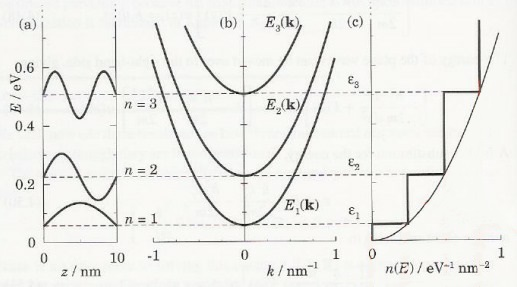
\includegraphics[width=\linewidth]{Images/QuantumWellDensityOfStates.png}
    \caption{Densità degli stati energetici in una QW in funzione dell'energia.}
    \label{fig:my_label}
\end{figure}

Il numero di eventi in cui un elettrone in banda di valenza assorbe un fotone della radiazione incidente effettuando una transizione in uno stato in banda di conduzione risulta essere proporzionale alla densità degli stati elettronici corrispondenti al valore energetico della transizione.
Come conseguenza di ciò l’andamento dello spettro di assorbimento rispecchierà ragionevolmente quello della densità degli stati in funzione dell’energia.

Nel Germanio la banda di valenza è generata dagli orbitali atomici di valenza di tipo \textit{p}. Sono quindi presenti tre differenti bande: lacune pesanti (HH), lacune leggere (LH) e Split-Off (SO). Le prime due sono degeneri in $\Gamma$, mentre la terza non lo è a causa dell'interazione spin-orbita. La massa effettiva delle lacune risulta essere differente nelle tre diverse bande. In virtù di ciò ogni banda genera differenti stati confinati in posizione $\Gamma$, indicati rispettivamente con HH$\textit{n}$, LH$\textit{n}$ e SO$\textit{n}$, dove $\textit{n}$ è il numero quantico che descrive l'eccitazione dello stato confinato. 

Analogamente con c$\Gamma\textit{n}$ e cL$\textit{n}$ si indicano gli stati elettronici confinati in banda di conduzione, rispettivamente in posizione $\Gamma$ e L.  Poiché il Germanio è un semiconduttore a gap indiretto, lo stato confinato fondamentale in banda di conduzione è cL1, il quale ha energia minore rispetto agli stati confinati c$\Gamma\textit{n}$.

Lo schema degli stati confinati nella buca quantica di elettroni e lacune calcolato a temperatura T = 0 è riportato in Fig.10.

\begin{figure}[h!]
    \centering
    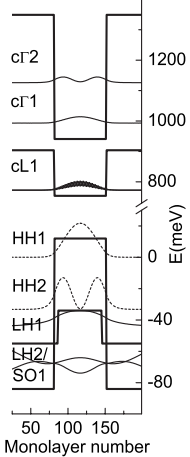
\includegraphics{Images/QWStates.png}
    \caption{Profili degli estremi della banda di valenza e di conduzione. Sono rappresentati i moduli quadri delle funzioni d'onda degli stati confinati degli elettroni e delle lacune. Autostati e autovalori energetici sono stati calcolati a temperatura nulla. Poichè gli spettri sono stati ricavati a temperatura ambiente ci si aspetta una diminuzione del gap interbanda di circa 0.1 eV.}
    \label{fig:my_label}
\end{figure}

L'assorbimento della radiazione incidente IR può essere attribuito alle transizioni di dipolo elettrico permesse tra gli stati confinati in banda di valenza e gli stati confinati in banda di conduzione: HH\textit{n}-c$\Gamma$\textit{n}, LH\textit{n}-c$\Gamma$\textit{n} e SO\textit{n}-c$\Gamma$\textit{n}. In base alle regole di selezione, fondate sulle leggi di conservazione, sono ammesse transizioni di dipolo elettrico solamente tra stati confinati nelle due bande aventi stesso numero quantico \textit{n}.

Sperimentalmente si osserva la presenza di distinti picchi nello spettro di trasmissione.

Tali picchi sono legati alla formazione di stati eccitonici (eccitoni), ovvero stati legati tra elettrone e lacuna generati dall'attrazione elettrostatica nel momento in cui la coppia viene creata dall'assorbimento di un fotone, generando un sistema idrogenoide. La formazione di un eccitone comporta la presenza di un'energia di legame tra le due particelle, che rende l'energia totale della coppia minore rispetto all'energia totale che si osserva in assenza della formazione dello stato legato. Questo fenomeno fa sì che i picchi delle transizioni che si osservano distintamente nello spettro, dovuti alla formazione di eccitoni nello stato di legame fondamentale, avvengano a energie inferiori rispetto all'energia di soglia della transizione tra stati confinati di valenza e di conduzione (l'energia di legame di un eccitone in questo tipo di strutture è nell'ordine della decina di meV).

Osservando lo spettro di trasmissione non si nota la presenza di assorbimento, aspettato tra i 0.7 e 0.8 eV, dovuto alle transizioni dagli stati confinati in banda di valenza in posizione $\Gamma$ e lo stato confinato in banda di conduzione in posizione L (cL1) pur essendo queste transizioni energeticamente favorevoli (richiedono meno energia) rispetto alle transizioni del gap diretto. Tali transizioni non vengono osservate nello spettro: esse sono estremamente meno probabili rispetto alle transizioni del gap diretto perché possono avvenire solamente nel momento in cui un elettrone interagisce simultaneamente con un fotone incidente e un fonone (processo a tre corpi), come conseguenza della conservazione dell'impulso del cristallo.
A causa di ciò, il coefficiente di assorbimento delle transizioni HH1-cL1, LH1-cL1 e SO1-cL1 è abbastanza basso da non renderle visibili nello spettro.

\subsection{Caratteristiche Specifiche degli Spettri.}

Comparando gli spettri di trasmissione dei due campioni 7909-3 e 7909-8 si nota come il primo picco presente negli spettri, dovuto alle transizioni tra stati eccitonici confinati HH1-c$\Gamma$1, avviene a 0.874$\pm$0.005 eV per il campione 7909-3 e a 0.860$\pm$0.006 eV per il campione 7909-8.
Questa differenza in energia indica che il campione 7909-3 presenta pozzi quantici più sottili rispetto al campione 7909-8, introducendo un maggiore grado di confinamento e un aumento della differenza energetica tra gli stati HH1 e c$\Gamma$1 nel pozzo quantico.

Lo spettro del campione 7909-8 presenta altri due distinti picchi alle energie di 0.897$\pm$0.008 eV e 0.955$\pm$0.012 eV. Essi sono dovuti rispettivamente alle transizioni tra stati eccitonici confinati HH2-c$\Gamma$2 e HH3-c$\Gamma$3. Questa identificazione è basata sull'osservazione del fatto che la densità ottica tende ad aumentare approssimativamente di uno stesso valore ($\sim$0.7) ogni qual volta è presente un picco. Questa caratteristica è associata a transizioni tra stati eccitonici confinati di una stessa serie (in questo caso HH$\textit{n}$-c$\Gamma\textit{n}$), in quanto, come precedentemente mostrato, l'andamento della densità ottica rispecchia quello della densità di stati elettronici in funzione dell'energia, la quale aumenta sempre di uno stesso valore ogni qual volta si raggiunge l'energia necessaria per osservare una nuova transizione della stessa serie.

Lo spettro del campione 7909-3 presenta altri due distinti picchi alle energie di 0.908$\pm$0.007 eV e 0.953$\pm$0.010 eV e uno meno marcato per 1.006$\pm$0.012 eV. Essi sono dovuti rispettivamente alle transizioni tra stati eccitonici confinati LH1-c$\Gamma$1, HH2-c$\Gamma$2, LH2-c$\Gamma$2. In questo campione, in cui è presente un maggior grado di confinamento, si osservano separatamente i primi picchi delle serie di transizioni HH$\textit{n}$-c$\Gamma\textit{n}$ e LH$\textit{n}$-c$\Gamma\textit{n}$. A differenza del campione 7909-8, nel campione 7909-3 è possibile fare questa identificazione in quanto l'aumento della densità ottica non è sempre lo stesso ogni volta che si presenta un picco nello spettro, ma ricorre un pattern preciso. Infatti l'incremento in OD tra la regione di trasparenza e il primo picco e tra il primo e il terzo picco è intorno a $\sim$0.6, che ci permette di identificare queste transizioni con 
le prime due della serie HH$\textit{n}$-c$\Gamma\textit{n}$. Lo stesso discorso vale per il secondo e il quarto picco delle transizioni, per cui si verifica un aumento in OD rispetto al picco precedente di $\sim$0.2 in ambo i casi, permettendoci di identificare queste transizioni con le prime due della serie LH$\textit{n}$-c$\Gamma\textit{n}$.

In ambo gli spettri non vi è evidenza della presenza di picchi dovuti alle transizioni tra stati eccitonici confinati SO$\textit{n}$-c$\Gamma\textit{n}$. Tali picchi possono essere evidenziati portando il campione a basse temperature.

Le incertezze sui valori energetici dei picchi di assorbimento sono state stimate mediante la HWHM dei picchi stessi.

\subsection{Confronto con l'Assorbimento di un Film Sottile in Germanio.}

Per concludere l'analisi si è determinato, con la stessa procedura sperimentale, lo spettro di trasmissione (e dunque le caratteristiche di assorbimento) di un film sottile in Germanio, con spessore pari a 8 $\mu$m, cresciuto a partire da un substrato in Silicio.
Lo spettro di trasmissione ottenuto, OD in funzione dell'energia della radiazione incidente, è riportato in Fig.11. Si è utilizzato un filtro neutro da 0.0025\% per ridurre l'intensità del fascio incidente e un filtro longpass RG-665. Inoltre poichè la misura in termini di OD è riferita allo spettro della sorgente, è stata effettuata una translazione dello spettro per trascurare i fenomeni di riflessione della radiazione in corrispondenza delle superfici del campione.

\begin{figure}[h!]
    \centering
    \includegraphics[width=\linewidth]{Images/SpettroFilmSottileGe_NoRiflessione.jpeg}
    \caption{Spettro di trasmissione di un film sottile in Germanio cresciuto su un substrato si Silicio.}
    \label{fig:my_label}
\end{figure}

Nell'immediatezza si nota come il film sottile risulta essere trasparente fino a circa 0.78 eV. A partire da questo valore energetico, l'assorbimento del film sottile aumenta sensibilmente rispecchiando l'andamento della densità degli stati elettronici in funzione dell'energia, il quale risulta proporzionale alla radice quadrata dell'energia stessa in un sistema in cui gli elettroni mantengono tre gradi di libertà spaziali (non sono soggetti al confinamento in strutture di dimensioni nanometriche).
Questi fenomeni di assorbimento sono legati alle transizioni da gap diretto del Germanio. Dallo spettro è possibile notare che la soglia di assorbimento risulta essere di circa 0.02 eV inferiore all'energy gap del Germanio a 300 K (0.8 eV). Tale comportamento è una diretta conseguenza del fatto che il film sottile in Germanio, cresciuto mediante tecniche di deposizione epitassiale su un substrato di Silicio, risulta essere sotto strain tensile a temperatura ambiente, il che ha l'effetto di diminuire il gap interbanda.

\section{Conclusioni}

Dai risultati emersi dagli spettri di assorbimento viene evidenziato il comportamento del Germanio come ottimo assorbitore. Questo lo si deduce dagli alti coefficienti di assorbimento corrispondenti alle transizioni tra stati confinati nelle QW. La struttura studiata ha elevate potenzialità applicative nell’ambito della costruzione di dispositivi utili nella fotonica, in particolare nella costruzione di modulatori elettro-ottici. In definitiva l’aspetto vantaggioso fondamentale rispetto a strutture simili che utilizzano altri semiconduttori, come ad esempio MQW in GaAs/AlGaAs, è quello di poter costruire tutta la struttura su di un substrato di Silicio, maggiormente utilizzato in microelettronica, mediante la tecnica dei substrati virtuali.

\section{Riferimenti}

\begin{itemize}
    \item \textit{Optical transitions in Ge/SiGe multiple quantum wells with Ge-rich barriers} - PHYSICAL REVIEW B 78, 041407(R) (2008)
    \item \textit{Electronic band structures of silicon–germanium (SiGe) alloys} - N. Moriù
    \item \textit{The physics of low-dimensional semiconductors - An introduction} - Ch.4 - John H. Davies - Glasgow University
    \item\textit{Fundamental Theory and Applications of FTIR Spectroscopy} - Jasco
\end{itemize}

\end{document}